\makeatletter\let\ifGm@compatii\relax\makeatother
\documentclass[utf8x,outline]{beamer}
\usepackage{default}

\usetheme{default}
\setbeamercolor{background canvas}{bg=black,fg=white}
\setbeamercolor{normal text}{fg=white}
\setbeamercolor{structure}{fg=white}

\usepackage[dutch]{babel}
\usepackage{graphicx}

\usepackage[official]{eurosym} % depens on: texlive-fonts-recommended
%~ \usepackage{amsmath}
%~ \usepackage{amssymb}
%~ \usepackage{tikz}

\title{Zelula slides}

\author{Group E}
\institute{TU Delft}
\date{\today}

\begin{document}

{
	\usebackgroundtemplate{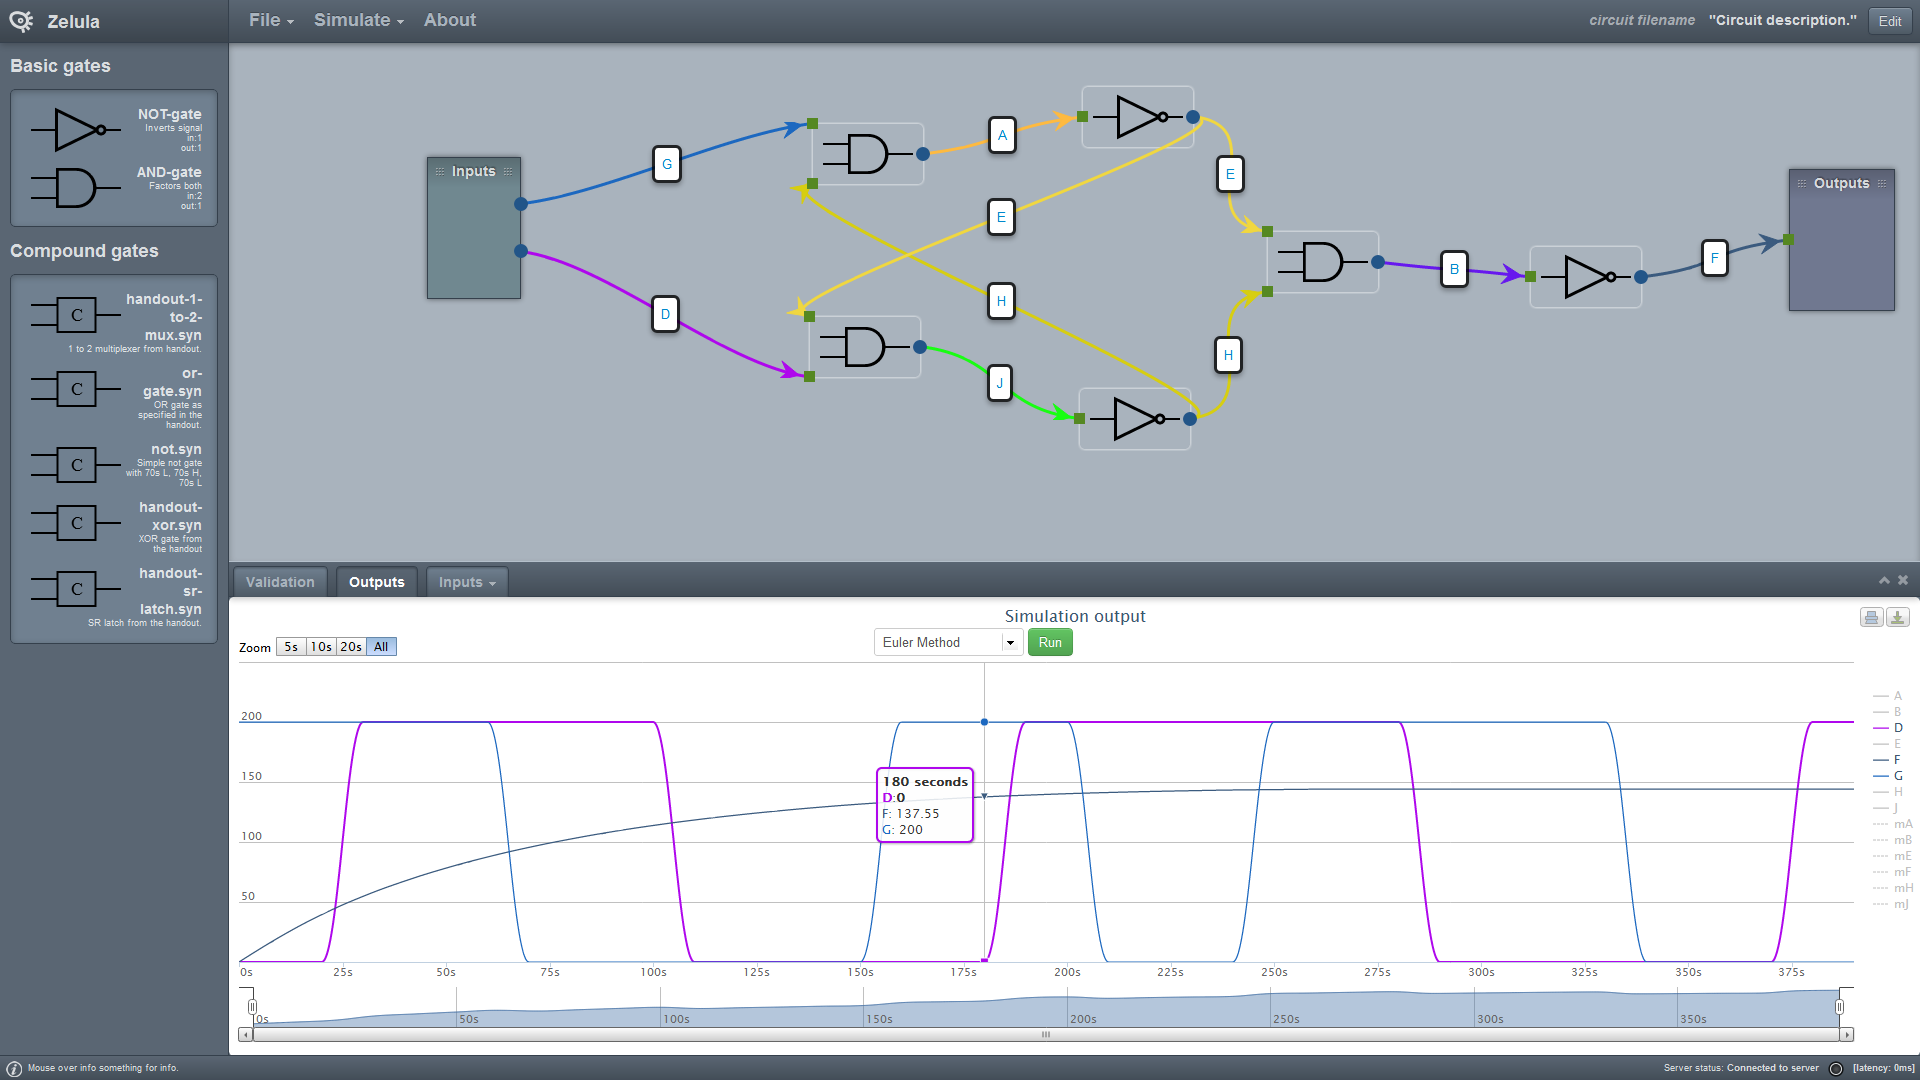
\includegraphics[width=1\paperwidth]{../../screenshots/final-1.png}}
	\begin{frame}[plain]{}
	\end{frame}
}
{
	\usebackgroundtemplate{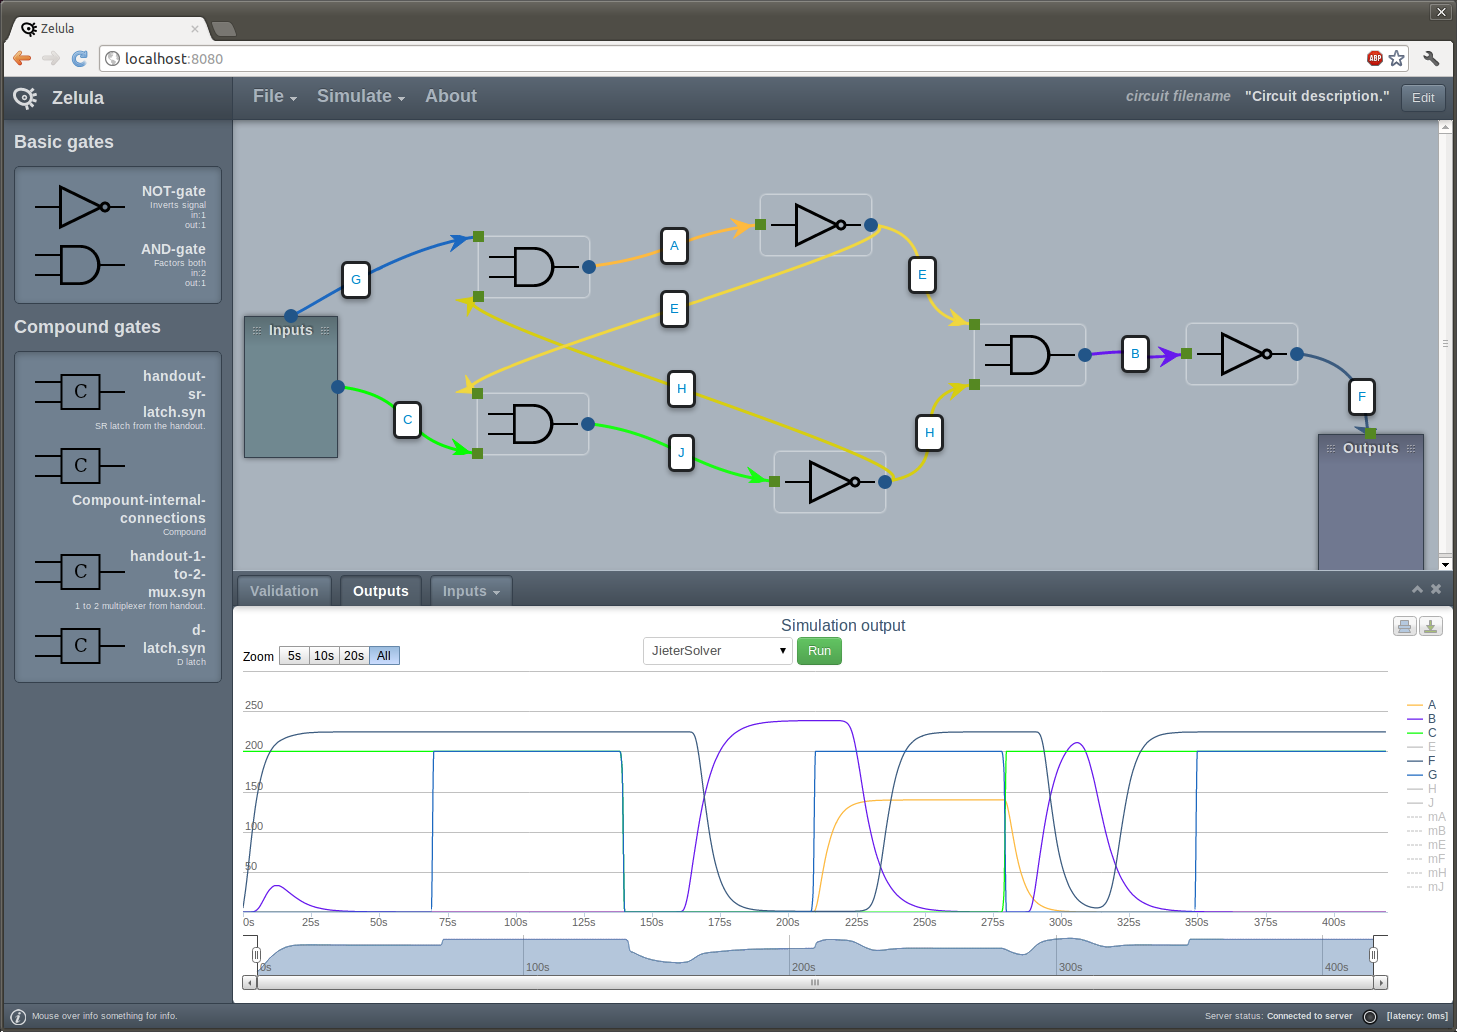
\includegraphics[width=1\paperwidth]{../../screenshots/showcase.png}}
	\begin{frame}[plain]{}
	\end{frame}
}
{
	\setbeamertemplate{navigation symbols}{}
	\usebackgroundtemplate{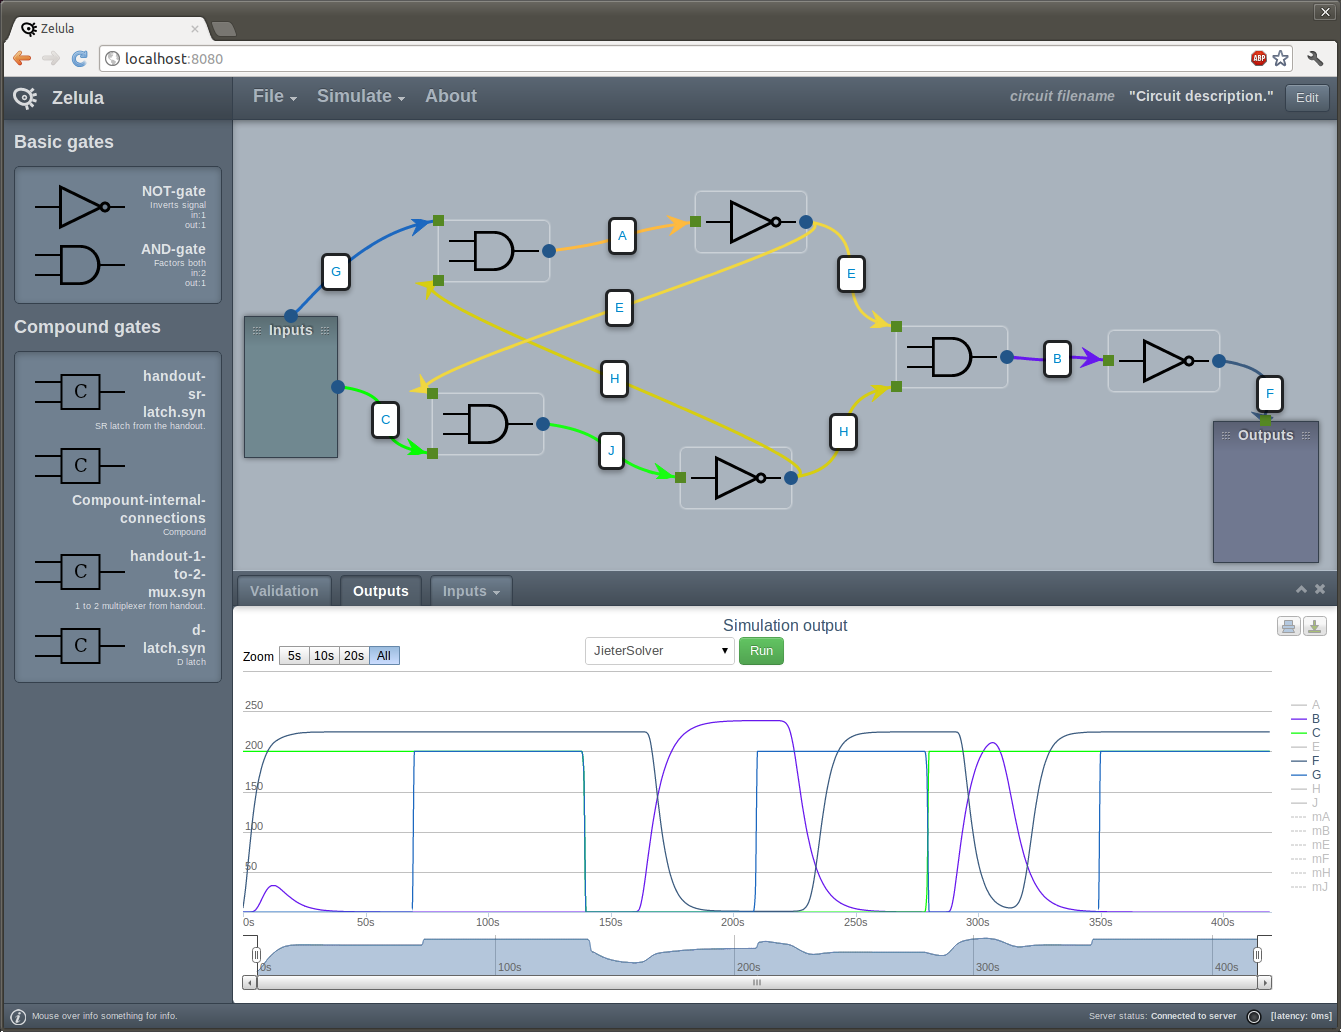
\includegraphics[width=1\paperwidth]{../../screenshots/showcase-1.png}}
	\begin{frame}[plain]{}
	\end{frame}
}

{
	\usebackgroundtemplate{
\includegraphics[width=1.5\paperwidth]{../../Presentation/zelula-bg.jpg}}%
	\begin{frame}{Zelula's key features}
		\begin{itemize}
			\item Intuitive interface:
			\begin{itemize}
				\item Drag \& Drop gates;
				\item Recognizable icons;
				\item Colored proteins;
			\end{itemize}
			\item Compound gates;
			\item Choose from 10 different solvers;
			\item Exportable to SBML;
			\item Platform independent:
			\begin{itemize}
				\item Client is in the browser;
				\item Works on tablets/phones.
			\end{itemize}
		\end{itemize}
	\end{frame}
}


\end{document}
